En esta sección se detallan las simulaciones hechas para validar el diseño de la red de compensación. En primer lugar, se simuló la respuesta del circuito con realimentación unitaria ante un escalón en la entrada, el cual caía de $\SI{30}{\volt}$ a $\SI{12}{\volt}$. Esta simulación se hizo para verificar si la realimentación unitaria era suficiente para compensar el lazo. La simulación se hizo para los siguientes valores de carga: $R_L = \{6,\ 30, \ 95\}\,\Omega$. Todas las simulaciones fueron hechas con el modelo promediado. 

\begin{figure}[H]
    \centering
    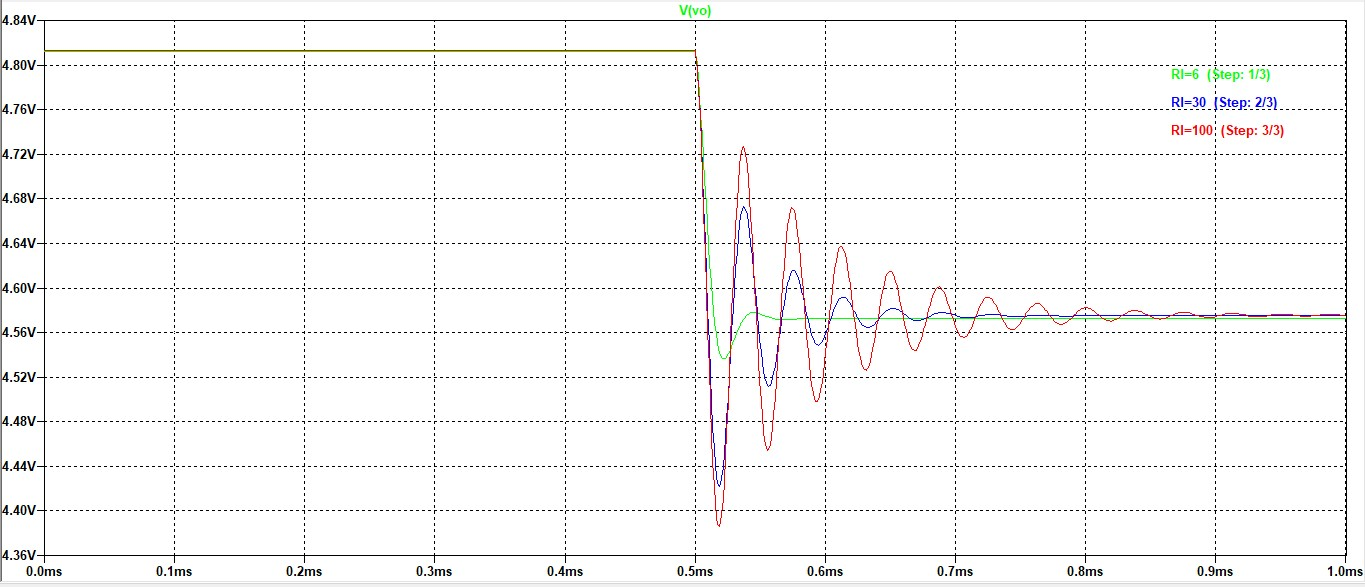
\includegraphics[width=0.9\textwidth]{img/simulacion imagenes/rta temporal-CL-sin compensar.png}
    \caption{Respuesta temporal sin compensar para distintos valores de carga.}
    \label{fig:rta temporal-sin compensar}
\end{figure}

Puede verse en la \autoref{fig:rta temporal-sin compensar} que la respuesta temporal depende fuertemente de la carga, como sugiere la ecuación del factor de calidad $Q$. Dado que la señal es excesivamente oscilante para ciertos valores de carga, es necesario compensar. Además, la salida no se establece en el valor deseado de $\SI{9.5}{\volt}$.

\begin{figure}[H]
    \centering
    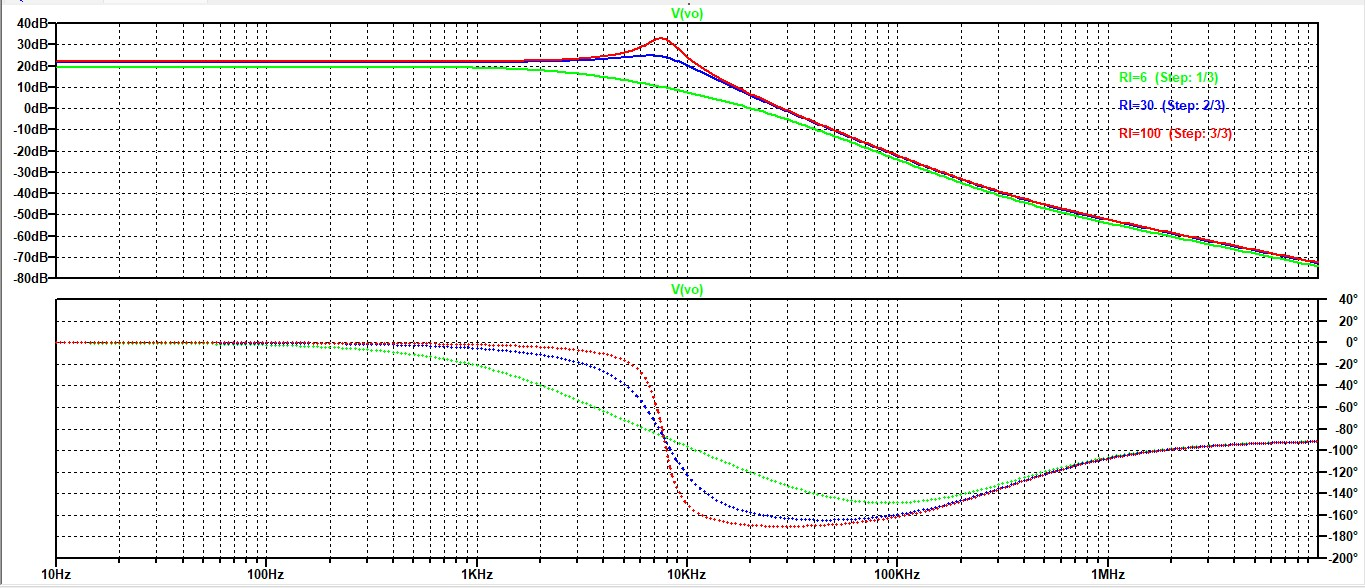
\includegraphics[width=0.9\textwidth]{img/simulacion imagenes/bode-OL.png}
    \caption{Diagrama de Bode a lazo abierto.}
    \label{fig:bode OL}
\end{figure}

La \autoref{fig:bode OL} muestra el diagrama de bode a lazo abierto de la \textit{buck}. Se destaca que a medida que la carga aumenta, el margen de fase decrece, como sugieren los resultados de la \autoref{fig:rta temporal-sin compensar}. Puede notarse el efecto de los polos complejos conjugados alrededor de la frecuencia $f = \SI{7}{\kilo \hertz}$. Estos polos imponen un cambio violento en la fase, lo que hace al sistema más oscilante.

\begin{figure}[H]
    \centering
    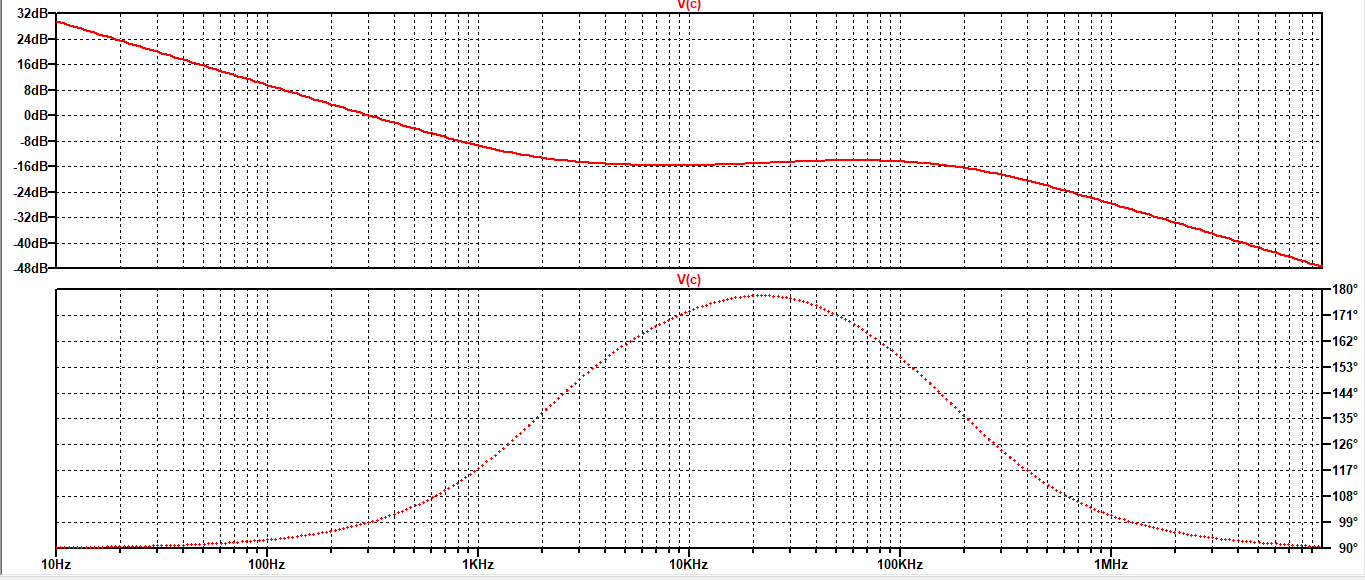
\includegraphics[width=0.9\textwidth]{img/simulacion imagenes/Bode-realimentador.png}
    \caption{Diagrama de Bode de la red de compensación.}
    \label{fig:bode realimentador}
\end{figure}

La \autoref{fig:bode realimentador} muestra el diagrama de Bode de la red de compensación. La misma fue diseñada con los criterios ya mencionados y de forma tal que añadiera fase para la frecuencia $f = \SI{7}{\kilo \hertz}$, mitigando así el efecto de los polos complejos conjugados.

\begin{figure}[H]
    \centering
    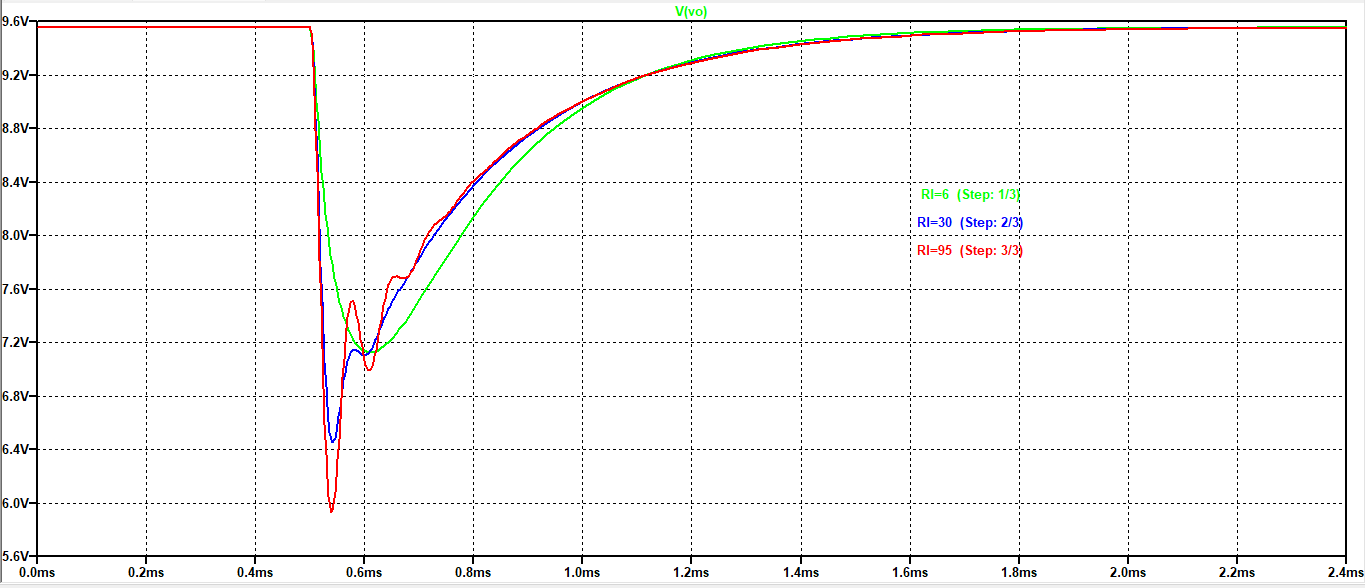
\includegraphics[width=0.9\textwidth]{img/simulacion imagenes/rta temporal-CL-compensado.png}
    \caption{Respuesta temporal del sistema compensado.}
    \label{fig:rta temporal comp}
\end{figure}

La \autoref{fig:rta temporal comp} muestra la respuesta del sistema compensado para el escalón ya mencionado. Se observa que se pudieron reducir las oscilaciones satisfactoriamente y que una vez agregada la compensación el sistema se establece en la tensión deseada. Si bien esta respuesta es un poco lenta, se considera que el tiempo de establecimiento es suficiente para esta aplicación.

\begin{figure}[H]
    \centering
    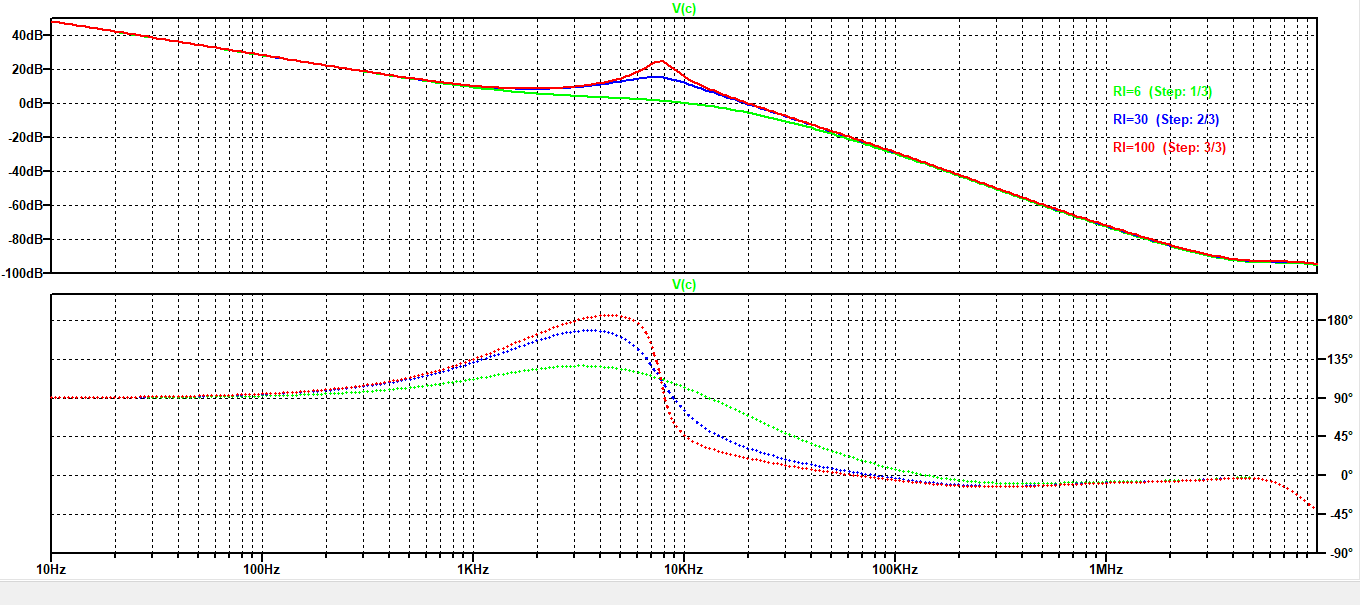
\includegraphics[width=0.9\textwidth]{img/simulacion imagenes/Bode-CL.png}
    \caption{Diagrama de Bode a lazo cerrado.}
    \label{fig:bode CL}
\end{figure}

La \autoref{fig:bode CL} muestra el diagrama de Bode a lazo cerrado para distintos valores de carga. Se observa que incluso en el peor de los casos el sistema presenta un margen de fase elevado (aproxiamdanete $\SI{100}{\degree}$). 